\chapter{Analýza a realizace klientské aplikace}

\todo{Doplnit kapitolu}

\section{Analýza uživatelů}

\subsection{Cílová zařízení}

Clientské webové aplikace jsou zpravidla zobrazovány běžnými uživateli v \gls{gui} prohlížečích na zařízeních s odlišnou velikostí monitoru. Dle statistik portálu StatCounter~\ref{pic:stats-devices} z hlediska zařízení používanými uživateli v posledních letech převládají mobilní zařízení.


\begin{fig:illustration}
   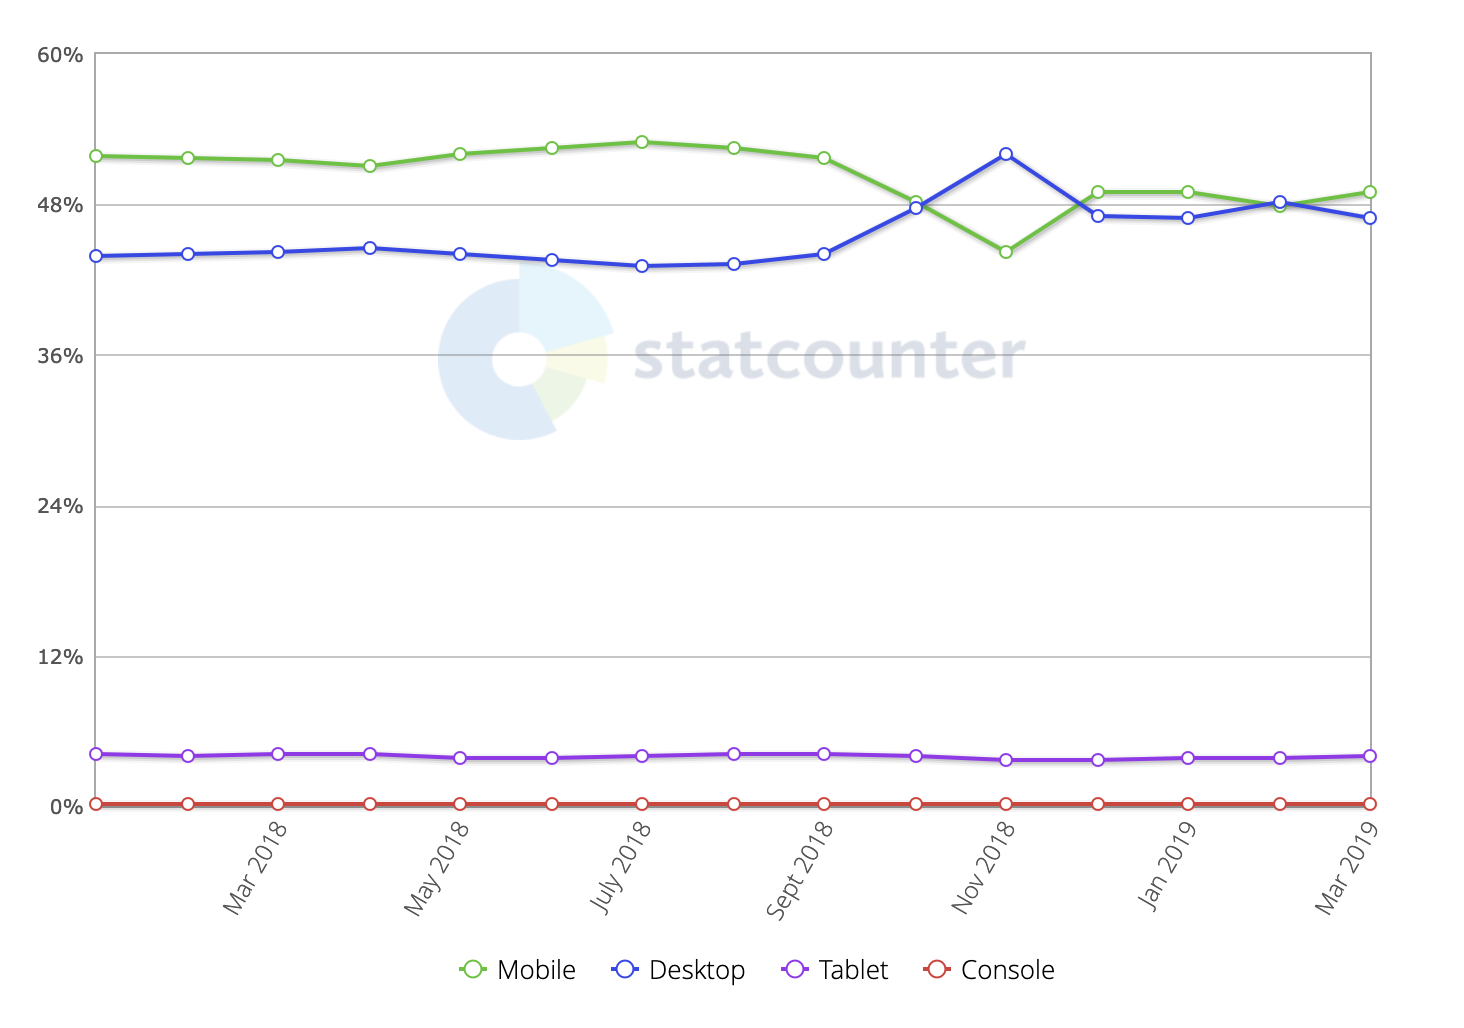
\includegraphics[width=1\textwidth]{images/stats-devices.png}
   \caption[Statistika zastoupení uživatelských zařízení]{Statistika zastoupení uživatelských zařízení 2018-01-01--2019-03-31 dle portálu StatCounter~\cite{statCounterDevices}}\label{pic:stats-devices}
\end{fig:illustration}
	


\section{Uživatelské rozhraní}

Na základě předchozích rozhodnutí o architektuře aplikace a realizace jednotlivých funkcionalit je navrženo vyhovující rozhraní. Základním východiskem je koncept minimalismu, jenž se projevuje ve snaze o zobrazení frekventovaných statistik a ovládacích prvků v přehledné formě a zároveň skrytí méně potřebných funkcionalit bez většího dopadu na komfortní ovládání aplikace.

Před vytvářením jednotlivých stránek je vytvořen grafický manuál~\footnote{Zde je přesnější anglický výraz \texttt{style guide}}. Jedná se o pomocnou stránku obsahující všechny základní prvky vyskutující se v designu -- barevná paleta, styly textů, nadpisy, prvky formulářů, apod.

\todo[color=colordiagram]{Ukázka části grafického manuálu}


\subsection{Zakládání projektů}
\todo[color=colordiagram]{WIREFRAME}

\subsection{Vyhledávání projektů}
\todo[color=colordiagram]{WIREFRAME}


